%
% fig-mercator.tex
%
% (c) 2025 Prof Dr Andreas Müller
%
\begin{figure}
\centering
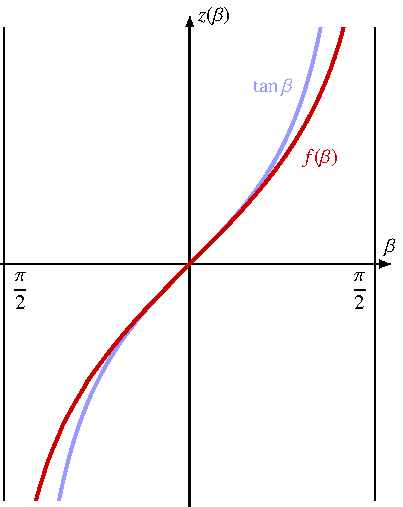
\includegraphics{chapters/030-kurvenintegral/images/mercator.pdf}
\caption{Die Funktion $f(\beta)$, die die Mercator-Projektion definiert,
dargestellt als die {\color{darkred}rote} Kurve.
Zum Vergleich ist auch die Funktion $\tan\beta$ darstellt, die zur
Zentralprojektion auf den Zylinder führt.
\label{buch:kurvenintegral:fig:mercator}}
\end{figure}
